\newcommand{\domain}{\operatorname{domain}}
\newtheorem{beispiel}{Beispiel}
\usetikzlibrary{decorations.markings}
%%
%% The next line says how the "vertex" style of nodes should look: drawn as small circles.
\tikzstyle{vertex}=[circle, draw, inner sep=0pt, minimum size=6pt]
%%
%% Next, we make a \vertex command as a shorthand in place of \node[vertex} to get that style.
\newcommand{\vertex}{\node[vertex]}


\chapterimage{chapter_head_1.png}

\chapter{Konsistenz und Suche}

\section{Einführung}\label{sec:einfuehrung}
	Wir haben bereits Probleme kennengelernt, wie beispielsweise das Einfärbeproblem von Landkarten, Kreuzworträtsel oder Sudokus. Das $n$-Damenproblem stellt die Frage, wie man $n$ Damen auf einem $n\times n$-Schachbrett stellen kann, sodass keine Dame von einer anderen geschlagen werden kann. Wir wollen in diesem Kapitel einfache Strategien kennenlernen, solche Probleme effizient mithilfe von \em Konsistenz und Suche \em zu lösen.
\section{Constraint Satisfaction Problem}
Alle die genannten Probleme können wir wie folgt Formalisieren:
\begin{definition}[Constraint Satisfaction Problem]
	Ein \em Constraint Satisfaction Problem \em (CSP) ist ein Tripel $P=\left(X,D,C\right)$, wobei
	\begin{itemize}
	\item $X = \left\{X_1, \dots, X_N\right\}$ eine endliche Menge von Variablen,
	\item $D = \left\{\domain(X_1),\dots, \domain(X_N)\right\}$ eine Menge der Domänen der Variablen in $X$, sowie
	\item $C = \left\{C_1,\dots,C_M\right\}$ eine endliche Menge von Contraints $C_i = \langle\left(\text{ Vars}, \text{Relation}\right)\rangle$ wobei \texttt{Vars} ein Tupel von Variablen ist, 	sowie \texttt{Relation} eine Relation zwischen den Variablen aus \texttt{Vars} ist.
	\end{itemize}
	Eine Belegung einer Variablen $X_i \in X$ heisst \em konsistent\em, falls sie keine der gegebenen Constraints verletzt. Eine Belegung aller Variablen heisst \em vollständig\em, ansonsten \em partiell\em. Eine Lösung eines Constraint Satisfaction Problems ist eine vollständige, konsistente Belegung.
\end{definition}
Wir können hierbei noch unterscheiden, zwischen
\begin{itemize}
	\item Unären Constraints, welche sich auf einzelne Variablen beschränken, wie beispielsweise $C_1 = \langle (X_1),X_1 \text{ist gerade}\rangle$,
	\item Binären Constraints, welche sich auf genau zwei Variablen bieziehen, wie $C_2 = \langle(X_1,X_2),X_1>X_2\rangle$, oder
	\item allgemein als $n$-äre Constraints, welche sich auf $n$ Variablen beziehen, wie $C_3 = \langle(X_1,\dots,X_n),\text{ Alle paarweise verschieden}\rangle$.
\end{itemize}

Wir können jedoch alle $n$-ären Contraints ($n>2$) auch als unäre oder binäre Constraints auffassen:

\begin{beispiel}
	Betrachte $C = \langle(X_1,X_2,X_3), \text{Alle paarweise verschieden}\rangle$. Wir führen eine Hilfsvariable $X_h$ ein, mit der Domäne
$$
	\domain(X_h) = \domain(X_1)\times \domain(X_2)\times\domain(X_3)
$$
	Nun können wir äquivalent zu $C$ die folgenden Constraints konstruieren:
\begin{align*}
	C_h &= \langle(X_h), (a,b,c)\in \domain(X_h) | a\neq b \wedge b \neq c \wedge a \neq c\rangle \\
	C_1 &= \langle(X_1,X_h), X_1 = X_h[0]\rangle \\
	C_2 &= \langle(X_2,X_h), X_2 = X_h[1]\rangle \\
	C_3 &= \langle(X_3,X_h), X_3 = X_h[2]\rangle
\end{align*}
wobei $X_h[k]$ für den $k$-ten Eintrag in der vektorwertigen Variable $X_h$ steht. In diesem konkreten Beispiel könnte man jedoch auch folgende Konstruktion wählen
\begin{align*}
	\hat{C}_1 &= \langle(X_1,X_2),X_1\neq X_2\rangle \\
	\hat{C}_2 &= \langle(X_2,X_3),X_2\neq X_3\rangle \\
	\hat{C}_3 &= \langle(X_1,X_3),X_1\neq X_3\rangle \\
\end{align*}
Jedoch demonstriert erstere Konstruktion, dass wir theoretisch von unären und binären Constraints ausgehen können. \\
Eine kleine Einschränkung jedoch ist, dass unsere Konsistenzalgorithmen sich eventuell anders verhalten können.

\end{beispiel}
Ein weiteres Beispiel für CSP sind Krypto-arithmetische Puzzle
\begin{beispiel}[Krypto-arthimetisches Problem]\label{cryptoarith}
	Gesucht ist eine paarweise unterschiedliche Belegung der Variablen \textbf{A}, \textbf{B}, \textbf{C}, so dass die Formel in Tabelle \ref{table:arithPuzzle} gilt.
	\begin{table}[h!]
\caption{Krypto-arithmetisches Puzzle}
		\centering
		\begin{tabular}{ll}\label{table:arithPuzzle}

		           & \textbf{A} \\
		+          & \textbf{B} \\ \hline
			\textbf{B} & \textbf{C} \\
		\end{tabular}
	\end{table}
	Mithilfe der Variable \textbf{U} können wir das Problem formalisieren. Dabei beachte, dass wir keine führenden Nullen zulassen wollen. Wir definieren also unsere Variablen

	\begin{align*}
		\domain(A) &= \domain(C) = \{0,1,2,3,4,5,6,7,8,9\} \\
		\domain(B) &= \{1,2,3,4,5,6,7,8,9\} \\
		\domain(U) &= \{0,1\}
	\end{align*} mit den Constraints
	\begin{align*}
		A + B &= C + 10 \cdot U \\
		B &= U \\
		A &\neq B \neq C
	\end{align*}
\end{beispiel}

\subsection{Konsistenz}
Um ein CSP zu lösen, können in der Regel bekannte Suchalgorithmen verwendet werden, jedoch bieten sich Algorithmen an, wie AC-3 oder Backtracking.
Fassen wir ein CSP als einen Graphen auf, bei dem die Knoten für die Belegungsmöglichkeiten der jeweiligen Variablen steht, die Kanten hingegen für die Constraint-Relationen, so können wir den AC-3 Algorithmus anwenden.
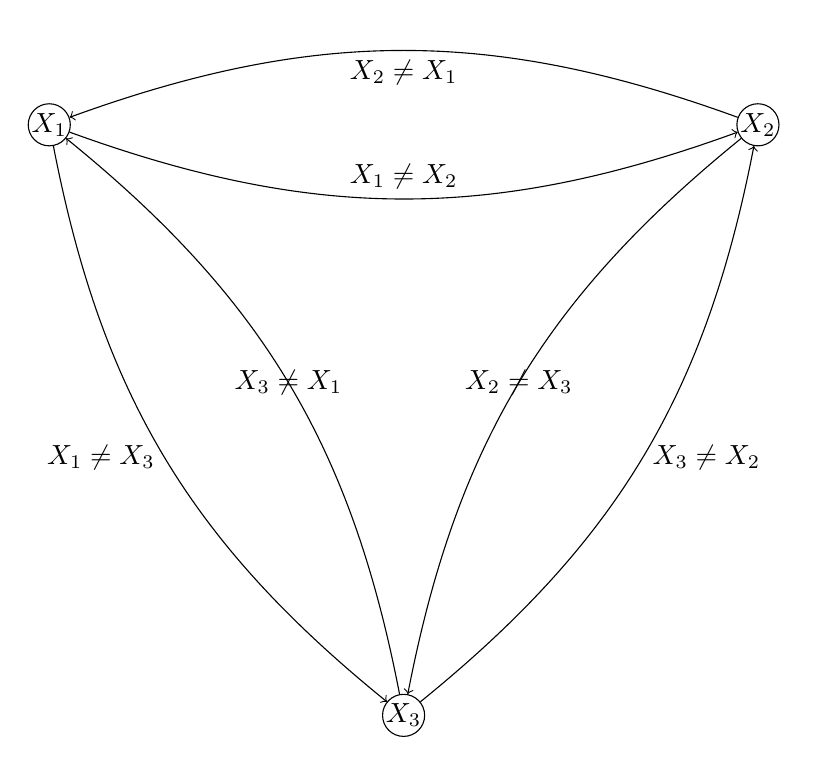
\begin{tikzpicture}[scale=1.5]
	\vertex (v) at (1, 5) [label=above:]{$X_1$};
	\vertex (x) at (7, 5) [label=right:]{$X_2$};
	\vertex (y) at (4, 0) [label=below:]{$X_3$};
	 \draw[->]
		(v) edge[bend right=20] node[above] {$X_1\neq X_2$} (x)
		(x) edge[bend right=20] node[below] {$X_2 \neq X_1$} (v)
		(x) edge[bend right=20] node {$X_2 \neq X_3$} (y)
		(y) edge[bend right=20] node[right] {$X_3 \neq X_2$} (x)
		(v) edge[bend right=20] node[left] {$X_1 \neq X_3$} (y)
		(y) edge[bend right=20] node {$X_3 \neq X_1$} (v)

	;
\end{tikzpicture}

Dazu definieren wir zuerst:

\begin{definition}[node- und arc-consistency]
	\begin{itemize}
		\item Eine Variable $X_i$ heisst \em node-consistent\em, wenn für alle möglichen Werte aus $\domain(X_i)$ alle unären Constraints auf $X_i$ erfüllen.
		\item Eine Variable $X_i$ heisst \em arc-consistent bezüglich der Variable \em$X_j$, wenn für alle $v \in \domain(X_i)$ ein $w \in \domain(X_j)$ existiert, sodass alle Constraints auf $(X_i,X_j)$ erfüllt sind.
		\item Ein CSP $P=(X,D,C)$ heisst \em arc-consistent\em, wenn alle Variablen in $X$ paarweise arc-consistent sind.
	\end{itemize}
\end{definition}
Der Arc-consistency Algorithmus (AC-3), welcher solche Graphen verwendet, findet Konflikte, die beim Belegen der Variablen per Backtracking auftreten und entfernt diese aus dem Suchraum.
Falls die Domänen verkleinert wurden, werden alle Kanten zu den benachbarten Knoten wieder überprüft. Der Algorithmus terminiert, da wir nur endlich viele Knoten und Kanten haben.
\begin{verbatim}
function AC3
 // Reduziert Domänen
     queue = Alle Kanten des CSP
     while (!empty(queue))
         Entferne eine Kante (x, y) aus queue;
         if(EntferneInkonsistenteWerte(x, y))
             foreach (Nachbar z von x)
                 queue.ADD(Kante(z, x))
end
function EntferneInkonsistenteWerte(x, y)
 // Liefert true, wenn Domäne D(x) reduziert wird
     removed = false
     foreach (Value v1 in D(x))
         if(Kein v2 in D(Y), so dass (x=v1, y=v2) alle Constraints
                                         zwischen (x,y) erfüllt)
             D(x).LÖSCHE(v1)
             removed = true
     return removed
end
\end{verbatim}
Wenn mindestens ein Wertebereich einer Variable leer ist, ist
offensichtlich keine vollständige Zuweisung und damit keine
Lösung mehr möglich.
Wenn alle Wertebereiche nur noch einen Wert enthalten, dann
können wir diese Werte als Zuweisung wählen und haben eine
Lösung gefunden. In den meisten Fällen werden wir aber um eine Suche nicht herum kommen, denn häufig bleiben mehrere Variablen in den Domänen übrig. \\
Wir wollen uns weiter mit Beispiel \ref{cryptoarith} befassen:
\begin{beispiel}
	Mit \em Backtracking-Search \em sieht man
	\begin{verbatim}
C ausgewählt
  C = 0 konsistent
    B ausgewählt
      B = 1 konsistent
        A ausgewählt
          A = 0 nicht konsistent (verletzt A != C constraint)
          A = 1 nicht konsistent (verletzt A != B constraint)
          A = 2 konsistent
            U ausgewählt
              U = 0 nicht konsistent (B = U)
              U = 1 nicht konsistent (A+B=C+10*U)
            U entfernt
          A = 3 konsistent
          ...
          A = 9 konsistent
            U ausgewählt
              U = 0 nicht konsistent
              U = 1 konsistent
              ergebnis <- C=0,B=1, A=9, U=1
\end{verbatim}
	Mit Forward-Checking verkleinern wir in jedem Schritt die Domäne der relevanten Variablen

\begin{verbatim}
C ausgewählt
  C = 0 konsistent
    FC: domain(A) = {1,2,3,4,5,6,7,8,9}
    B ausgewählt
      B = 1 konsistent
        FC: domain(A) = {2,3,4,5,6,7,8,9}, domain(U) = {1}
        A ausgewählt
          A = 2 konsistent (hier kein A=0,1)
            FC: domain(U) = {}, backtrack
          A = 3 konsistent
          ...
          A = 9 konsistent
            FC: keine Änderung
            U ausgewählt
              U = 1 konsistent (U=0 kommt nicht vor)
              ergebnis <- C=0, B=1, A=9,U=1
\end{verbatim}

\end{beispiel}

\section{Mit Prolog CSPs lösen}
(SWI-)Prolog ist eine logische Programmiersprache, welche per Backtracking aus einer Wissensdatenbank und Termen CSPs bedingt lösen kann.
\subsection{SWI-Prolog}
Mit dem Standardrepertoire von SWI-Prolog wollen wir beispielsweise das Crypto-Arithmetische Rätsel in Tabelle \ref{SENDMORY}
\begin{table}[!h]
\centering
\caption{Send More Money}
\label{SENDMORY}
\begin{tabular}{lllll}
\textbf{}  & \textbf{S} & \textbf{E} & \textbf{N} & \textbf{D} \\
+ & \textbf{M} & \textbf{O} & \textbf{R} & \textbf{E} \\\hline
\textbf{M} & \textbf{O} & \textbf{N} & \textbf{E} & \textbf{Y}
\end{tabular}
\end{table}
lösen, dann beschreiben wir das Problem beispielsweise durch
\begin{verbatim}
gen([S,E,N,D,M,O,R,Y]) :-
  permutation([S,E,N,D,M,O,R,Y,_,_],[0,1,2,3,4,5,6,7,8,9]).
gl1([S,E,N,D,M,O,R,Y]) :-
        1000*S+100*E+10*N+D
       +1000*M+100*O+10*R+E =:=
10000*M+1000*O+100*N+10*E+Y.

lsg :- gen([S,E,N,D,M,O,R,Y]),gl1([S,E,N,D,M,O,R,Y]).
\end{verbatim}

In dieser Version liefert uns Prolog keine explizite Belegung der Variablen, jedoch erhalten wir die Bestätigung
\begin{verbatim}?- lsg.
true\end{verbatim}
Leider akzeptiert der \texttt{=:=} Operator auf der rechten Seite keine freien Variablen, weshalb hier das Prädikat \texttt{gen} unabdingbar ist. Wir können in Prolog jedoch das Modul
\texttt{clpfd} verwenden.
\subsection{CLP(FD)}
Constraint Logic Programming over Finite Domains verwendet, anders als Prolog, nun Konsistenzalgorithmen, um die Domänen der Variablen sukzessive zu verkleinern, und somit den Suchraum zu verkleinern.
In Prolog mit CLP(FD) sieht unser Puzzle nun wie folgt aus:

\begin{verbatim}
:- use_module(library(clpfd)).

sendmore([S,E,N,D,M,O,R,Y]) :-
        Vars=[E,N,D,O,R,Y],
        Vars ins 0..9,
        S in 1..9,
        M in 1..9,
        all_different([S,E,N,D,M,O,R,Y]),
        1000*S+100*E+10*N+D
       +1000*M+100*O+10*R+E #=
10000*M+1000*O+100*N+10*E+Y.
\end{verbatim}
Tatsächlich erhalten wir damit das Ergebnis
\begin{verbatim}
?- sendmore([S,E,N,D,M,O,R,Y]).
S = 9,
M = 1,
O = 0,
E in 4..7,
all_different([9, E, N, D, 1, 0, R, Y]),
91*E+D+10*R#=90*N+Y,
N in 5..8,
D in 2..8,
R in 2..8,
Y in 2..8.
\end{verbatim}
Wir haben also die Domänen eingeschränkt, aber existiert tatsächlich eine Lösung unseres Puzzles? Wollen wir eine explizite Lösung erhalten, so verwenden wir \texttt{labeling}.
\begin{verbatim}
26 ?- sendmore([S,E,N,D,M,O,R,Y]),label([ff],[S,M,O,E,N,D,R,Y]).
S = 9,
E = 5,
N = 6,
D = 7,
M = 1,
O = 0,
R = 8,
Y = 2 ;
\end{verbatim}

\texttt{labeling} zwingt Prolog nun die Variablen zu benennen. Dazu stehen einige verschiedene Suchstrategien zur Verfügung. \newpage

\begin{table}[]
\centering
\begin{tabular}{lll}
Variablen   &                   &                                                                                                \\
            & \textbf{leftmost} & Die Variablen werden von links nach rechts durchgegangen (default)                             \\
            & \textbf{ff}       & First Fail. Belegt Variablen mit der kleinsten Domäne zuerst. \\
            & \textbf{ffc}      & Belegt Variablen mit der kleinsten Domäne und mit den meisten \\ & & Constraints zuerst.              \\
            & \textbf{min}      & Die Variable mit der kleinsten unteren Schranke wird zuerst belegt.                            \\
            & \textbf{max}      & Die Variable mit der kleinsten unteren Schranke wird zuerst belegt.                            \\
Werte  & &\\     & \textbf{up}       & Aufsteigend (default)                                                                          \\
            & \textbf{down}     & Absteigend                                                                                     \\
Verzweigung &                   &                                                                                                \\
            & \textbf{step}     & Für jede Variable X entscheide zwischen X=V und X!=V (default)                                 \\
            & \textbf{enum}     & Multiple Entscheidung für ein X entsprechend seiner Domäne                                     \\
            & \textbf{bisect}   & Entscheidet zwischen X<=M und X>M, mit Mittelpunkt M der \\ &  & Domäne
\end{tabular}
\end{table}
Verschiedene CSPs benötigen verschiedene Strategien, um möglichst effizient eine Lösung zu finden.

\begin{thebibliography}{999}
\bibitem [JS] AJoshua Schmidt, Constraint Logic Programming: Konsistenz und Suche, 31.05.2016
\bibitem [TR] ATobias Rosenkranz, Konsistenz und Suche, 06.06.2017
\end{thebibliography}
